\documentclass[../_main/handlingar.tex]{subfiles}

\begin{document}
\proposition{Uppfräschning av gamla arkivet}
Redan förra året valde styrelsen att flytta arkivet från andra våningen till Tyskland med tanken att det rummet skulle kunna användas som mötesrum och som ett Phøsrum under nollningen. Eftersom rummet för tillfället saknar lämpligt möblemang etc. till ändamål för detta syftet vill vi därför köpa ny inredning passande rummets funktionalitet både som mötesrum och Phøsrum. Bilden nedan är ett förslag på hur rummet ska utformas men inte begränsat till det.

\begin{center}
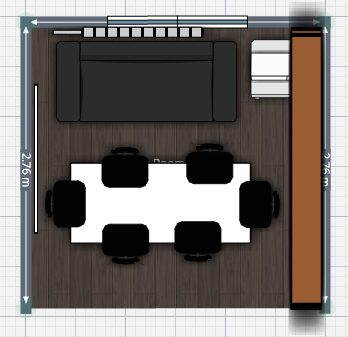
\includegraphics[width=10cm]{arkivet.png}
\end{center}

Därför yrkar vi på
\begin{attsatser}
    \att köpa in ny inreding samt nödvändiga inventarier till rummet.
    \att bugeten för projektet sätts till 10000kr.
    \att kostnaden belastar utrustningsfonden.
    \att detta läggs på beslutsuppföljningen till HT/16 där sittande styrelsen står som ansvarig.
\end{attsatser}

\begin{signatures}{2}
    \ist
    \signature{Anders Nilsson}{Förvaltningschef}
    \signature{Molly Rusk}{Øverphøs}
\end{signatures}

\end{document}
